% tex file for hypothesis testing results
\par \indent The results of our simple linear regression t-statistic 
comparisons across subjects are shown in [Figure \ref{fig:mask}]. We can see 
each slice of the brain from top to bottom in each section of the image. The 
blue areas shows parts of the brain that had a negative t-statistic while the 
red parts of the image shows parts of the brain that had a positive t-
statistic.

\begin{figure}[ht]
\centering
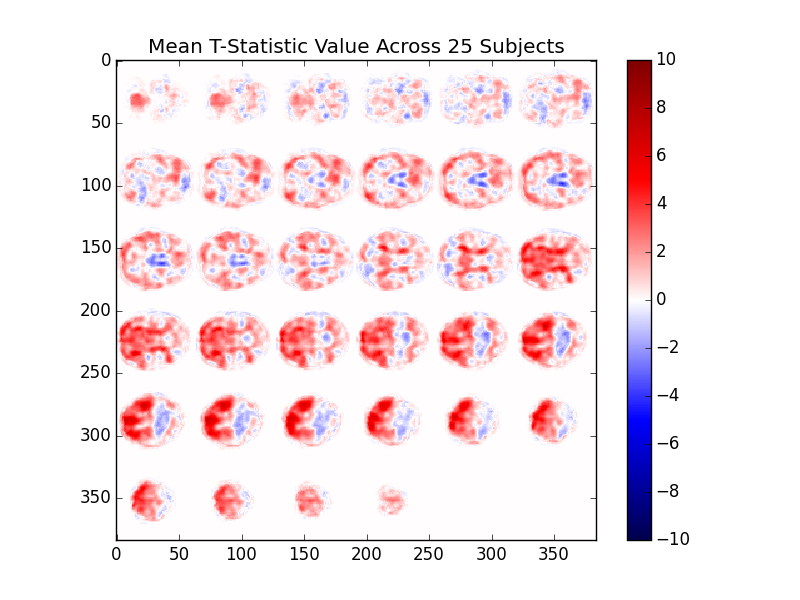
\includegraphics[scale=0.5]{images/hypothesis_testing}  
\caption{Across-subject mean of t-Statistic per voxel.}
\label{fig:mask}
\end{figure}

\par The parts of the image that were cut out by the mask are white so we can 
more clearly see the contrast in our results. Based on a cursory look at this 
image, we can see a pattern of dark blue areas in the left middle parts of 
the brain, and area of dark red in the center middle parts parts of the 
brain. 
